\documentclass[a4paper,10pt]{article} % na razie jako article, jak będzie więcej treści zmieni się na report.

\usepackage[polish]{babel}
\usepackage[utf8]{inputenc}
\usepackage{polski}
\usepackage[T1]{fontenc}

\usepackage{indentfirst}
\usepackage{amsmath, amstext} % ,amsfonts,amssymb
\usepackage{verbatim}
\usepackage{booktabs}
\usepackage{color}
\usepackage[usenames,dvipsnames,svgnames]{xcolor}
\usepackage{utopia}
\usepackage{geometry}
\geometry{verbose,lmargin=3cm,rmargin=3cm}
\frenchspacing

\usepackage{graphicx}

% podtytuł
\usepackage{titling}
\newcommand{\subtitle}[1]{
 \posttitle{
  \par\end{center}
  \begin{center}\large#1\end{center}
  \vskip0.5em}
}

%opening
\title{Nowe Trendy w Obliczeniach Neuronowych}
\subtitle{Spike and Slab Restricted Boltzmann Machine w klasyfikacji obiektów ze zbioru CIFAR-10}
\author{Konrad Brus \\ Jakub A. Gramsz}

\begin{document}
\maketitle

\begin{abstract}
Projekt ma na celu implementację Gaussian Restricted Boltzmann Machine oraz Spike and Slab RBM (zaprezentowanych w \cite{courville2013spike}) i wykorzystanie ich do klasyfikacji obiektów przedstawionych na obrazach. Implementacja uczona oraz testowana będzie na zbiorze danych CIFAR-10 (przedstawiony w \cite{cifar}) przy wykorzystaniu algorytmu uczenia Contrastive Divergence.
\end{abstract}

\section{Wstęp teoretyczny}
Maszyna Boltzmanna (ang. \textit{Boltzmann Machine}, BM) jest nieskierowanym grafem probabilistycznym z
węzłami o wartościach dyskretnych lub ciągłych. Model BM można interpretować jako stochastyczną sieć
neuronową, w której stan każdego neuronu zależy od neuronów do niego połączonych. Początkowo
zaproponowano maszynę Boltzmanna jako graf pełny z neuronami o wartościach binarnych, taka sieć była
analogiczna do sieci Hopfielda jeżeli zastosowalibyśmy neurony deterministyczne zamiast stochastycznych.

\section{Opis zbioru danych}
Do badań zostanie użyty zbiór CIFAR-10. Zawiera on 60000 kolorowych obrazów o wymiarach 32x32 pikseli, należących do jednej z 10 klas: 
\begin{itemize}
	\item airplane, automobile, bird \\
	\begin{center} 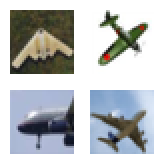
\includegraphics{imgs/class_0.png} 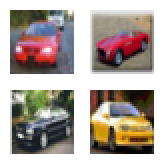
\includegraphics{imgs/class_1.png} 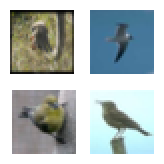
\includegraphics{imgs/class_2.png} \end{center}

	\newpage

	\item cat, deer, dog \\
	\begin{center} 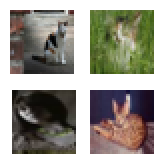
\includegraphics{imgs/class_3.png} 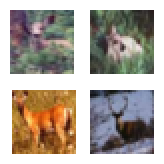
\includegraphics{imgs/class_4.png}  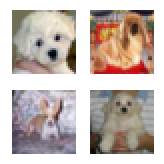
\includegraphics{imgs/class_5.png} \end{center}

	\item frog, horse, ship \\
	\begin{center} 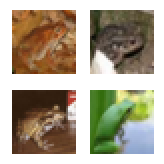
\includegraphics{imgs/class_6.png} 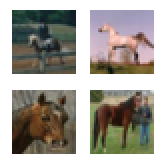
\includegraphics{imgs/class_7.png}  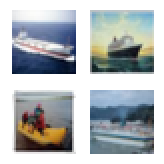
\includegraphics{imgs/class_8.png}  \end{center}

	\item truck \\
	\begin{center} 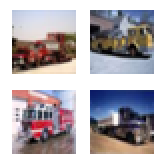
\includegraphics{imgs/class_9.png} \end{center}
\end{itemize}

Na jedną klasę przypada 6000 obrazów.

Zbiór jest wstęnie podzielony na dwie części - treningową (zawierającą 50000 obrazów, 5000 na klasę) oraz walidacyjną (10000 obrazów, 1000 na klasę).


\section{Opis problemu}

\section{Opis modelu}

\section{Opis algorytmu uczenia}

\section{Opis eksperymentu (zbioru danych)}

\section{Dostrajanie modelu i wyniki}

\section{Dyskusja i wnioski}


\bibliographystyle{abbrv}
\nocite{*} % na razie póki mało co jest cytowane (powoduje że wszystko z listy artykułów jest tu widoczne
\bibliography{lit}

\end{document}
